\subsection{Relational learning across tasks for SET cards}
\label{ssec:set_exp}
\def\attr#1{{\small\texttt{#1}}}
\def\mattr#1{{\mbox{\footnotesize\texttt{#1}}}}

In this set of experiments we study an Abstractor's ability to apply relations learned in one task to a different task. 
As described in Section~\ref{ssec:set} the game SET involves several levels of abstraction over sensory embeddings.
Cards vary along the four attributes \attr{color}, \attr{number}, \attr{pattern}, and \attr{shape}, 
as shown in Figure \ref{fig_set}a). The task requires use of an AAB rule: Along each dimension, three cards in a set must either have the same or unique values. As examples, if we denote this function as $f_\mattr{attr}(x_1, x_2, x_3)$ 
for an attribute \attr{attr}, then the first three cards in each of the three rows of cards in Figure \ref{fig_set} 
(reproduced below) have the following values $(f_\mattr{number}, f_\mattr{color}, f_\mattr{pattern}, f_\mattr{shape})$:
\begin{center}
	\begin{tabular}{cc}
	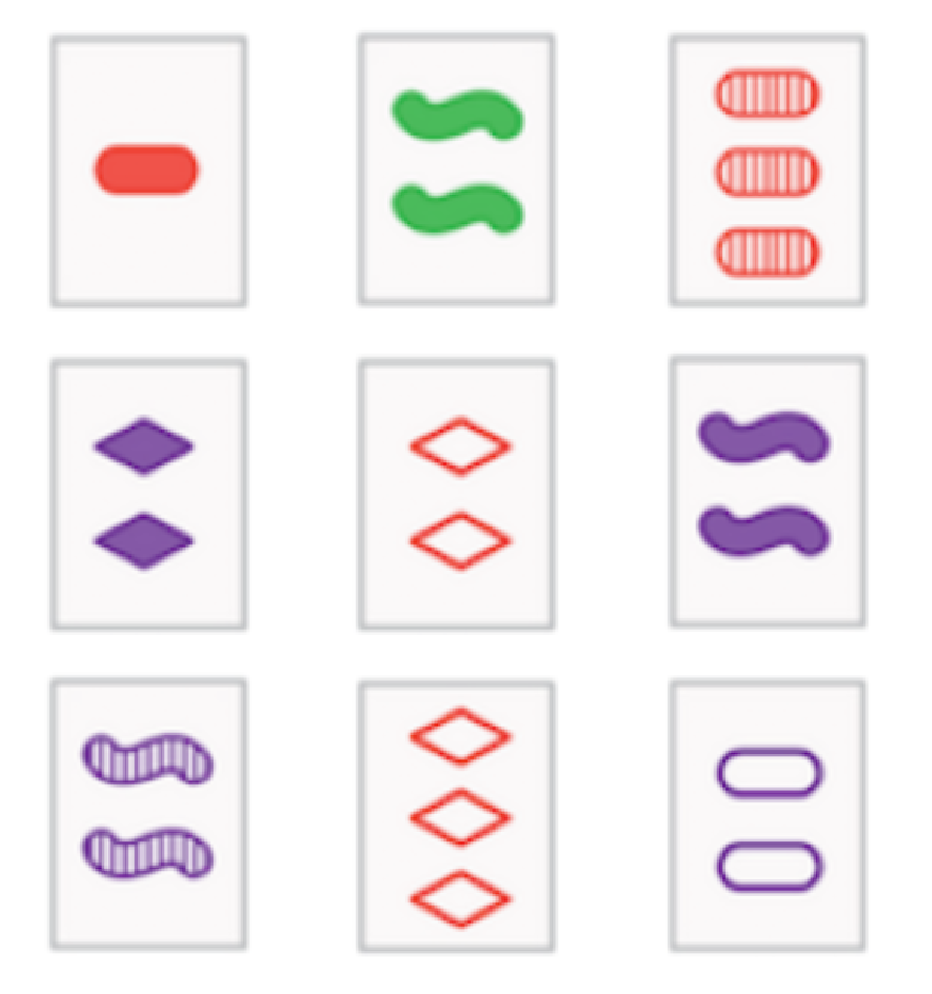
\includegraphics[width=.18\textwidth]{figures/set/set_example2}&\\[-1.35in]
	& \renewcommand{\arraystretch}{2}
	\begin{tabular}{c}
     (1, 0, 0, 0) \\
	 (1, 0, 0, 0) \\
	 (0, 0, 0, 1) 
	\end{tabular}
	\end{tabular}
\end{center}

To simulate this task we first train a convolutional neural network to process the color images 
of the cards (a full deck includes 81 cards). The CNN is trained to predict the attribute of 
each card, as a multi-label classification, and then an embedding of dimension $d=32$ of 
each card is obtained as a fixed input vector. 

\subtask{Same/Different task} We train a first Abstractor on a Same/Different task, 
where for a training set of pairs of cards, the Abstractor predicts whether the cards are 
the same or different in each of the four attributes. The Abstractor is trained with 
four relational cross attention heads on this task.

\begin{figure}[t!]
	\begin{center}
	\begin{tabular}{cc}
		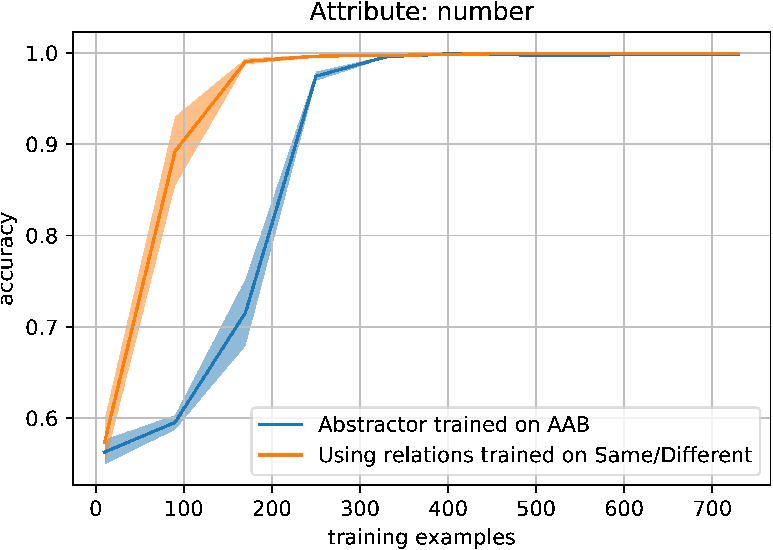
\includegraphics[width=.42\textwidth]{figures/set/AAB_comparison_number-crop} &
		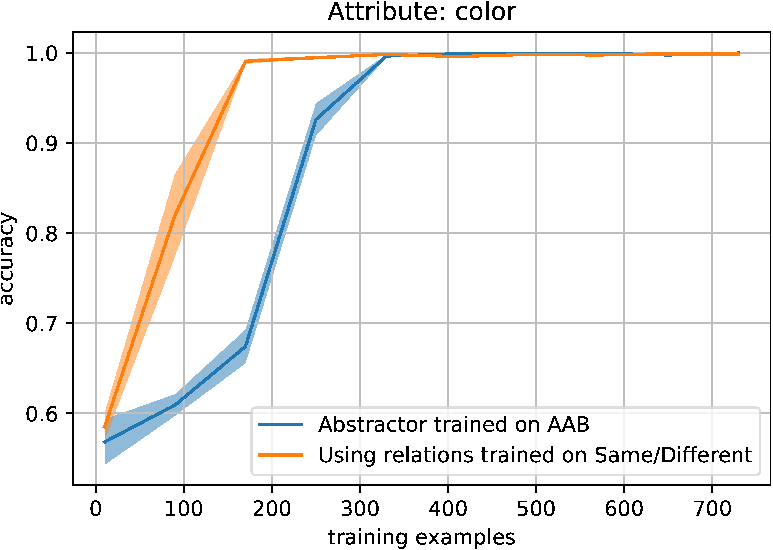
\includegraphics[width=.42\textwidth]{figures/set/AAB_comparison_color-crop} \\
		&\\
		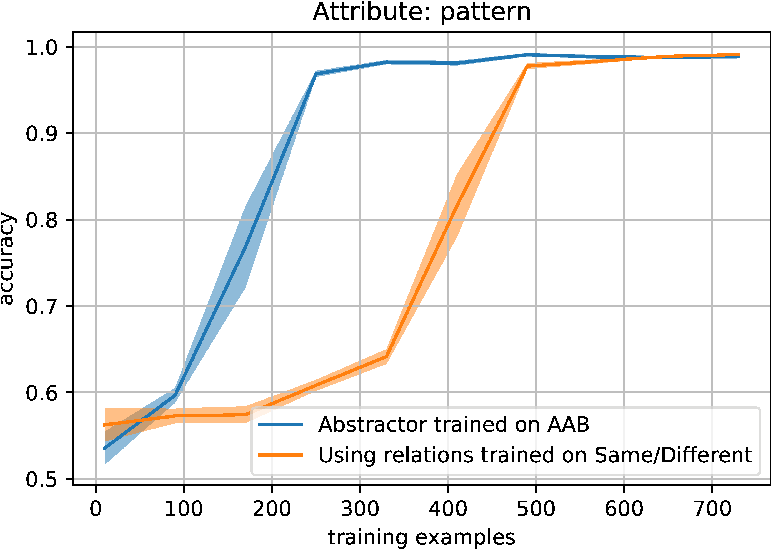
\includegraphics[width=.42\textwidth]{figures/set/AAB_comparison_pattern-crop} &
		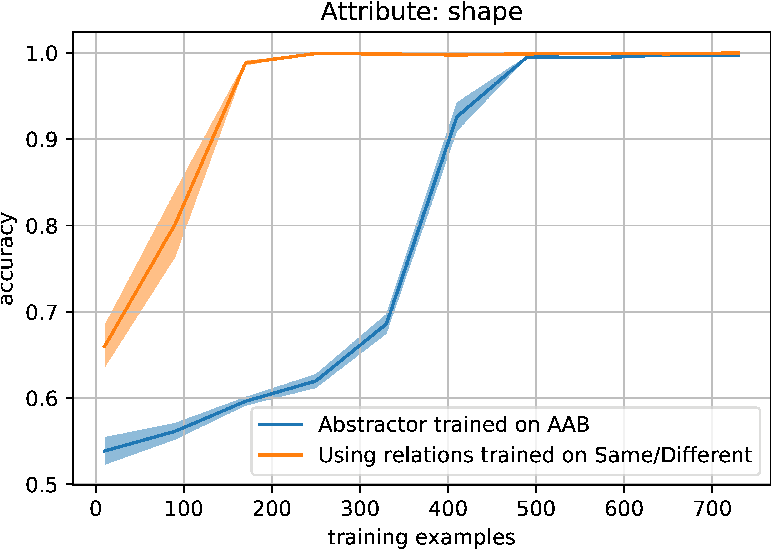
\includegraphics[width=.42\textwidth]{figures/set/AAB_comparison_shape-crop}
	\end{tabular}
	\caption{Learning curves on the SET relation learning task for all four attributes: \attr{number}, \attr{color}, \attr{pattern}, and \attr{shape}.  An Abstractor model was first trained on the Same/Different task, as a multi-label classification task across all four attributes, using four relational cross attention heads. The input to model is embeddings from a convolutional neural network trained on images. Two Abstractors were then trained: an Abstractor was trained from scratch on the AAB task, and another Abstractor was trained but with the relational cross attention heads initialized and fixed to be those learned in the Same/Different task--only the \MLP to classify the abstract states was trained. The lines indicate the mean AAB classification accuracy over 10 trials for that training set size, and the shaded region indicates the standard error of the mean.}
	\label{fig:aab_learning_curves}
    \end{center}
\end{figure}

\subtask{AAB task} Next, we train Abstractors separately for each of the four attributes. 
Here the task is to predict whether an input triple of cards is valid for that attribute. 
If the triple forms an AAB pattern, the class label is zero; if the triple forms an ABC 
pattern or an AAA pattern, the class label is one. For each attribute we train 
two different Abstractors---the first is trained from scratch, and includes the learning 
of four new relational cross attention heads. The second Abstractor is 
initialized so that the attention heads are given by the Abstractor learned for the 
Same/Different task. Thus, only the \MLP used to classify the abstract state $A$ is 
learned for this task.

\subtask{Evaluation} We evaluate learning curves on the AAB tak for each 
model and attribute, for training set sizes ranging from $10$ triples to $1,000$ sequences in increments of $100$. For each training set size we run 10 trials each. Each trial consists of training a model on a dataset of the corresponding size for 50 epochs. For each trial, we evaluate the classification 
accuracy on an independent test sample of $500$ triples of card images. The results are shown 
in Figure~\ref{fig:aab_learning_curves}

